% Generated by tools/paper/render.py from main_text.py; edit the source there, not this file.
\begin{figure*}[t]
\centering
\resizebox{\textwidth}{!}{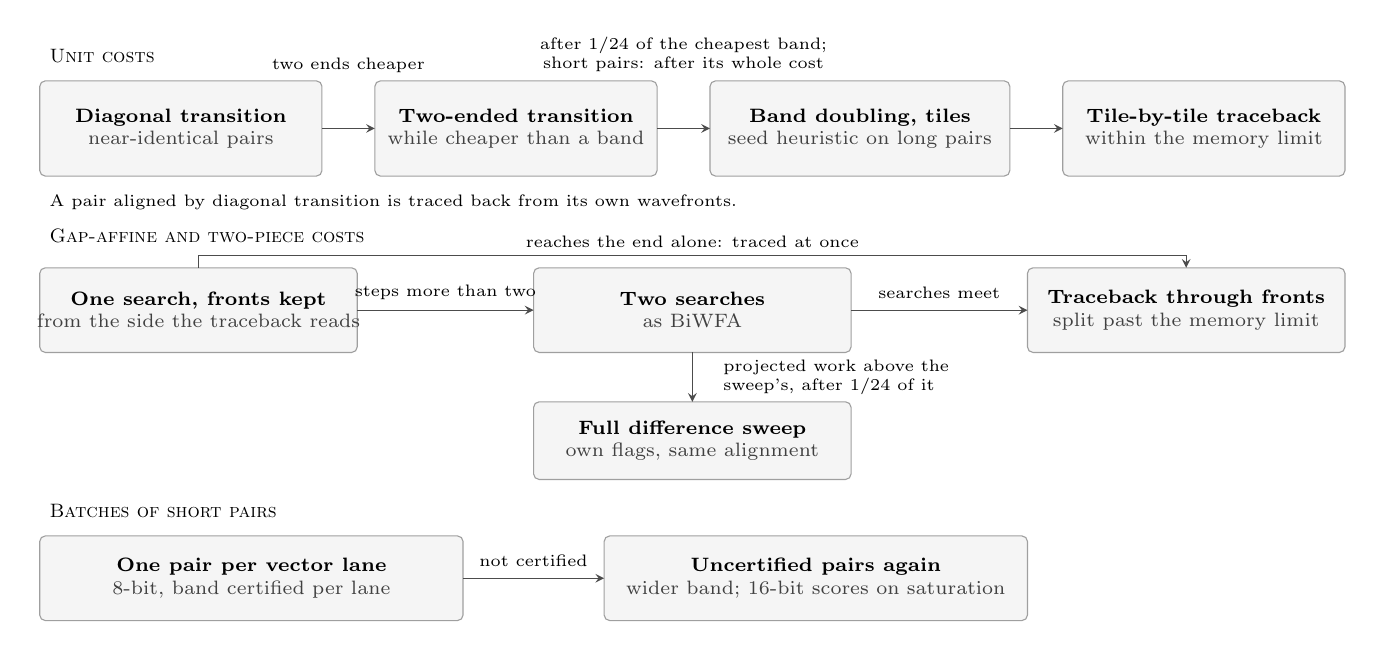
\begin{tikzpicture}
\node[anchor=west,font=\scriptsize\scshape] at (0.224,-0.224) {Unit costs};
\node[anchor=west,font=\scriptsize\scshape] at (0.224,-2.509) {Gap-affine and two-piece costs};
\node[anchor=west,font=\scriptsize\scshape] at (0.224,-6.003) {Batches of short pairs};
\draw[rounded corners=2pt,fill=gray!8,draw=gray!75] (0.224,-0.538) rectangle (3.808,-1.747);
\node[align=center,font=\scriptsize] at (2.016,-1.142) {\textbf{Diagonal transition}\\{\color{black!75}near-identical pairs}};
\draw[rounded corners=2pt,fill=gray!8,draw=gray!75] (4.480,-0.538) rectangle (8.064,-1.747);
\node[align=center,font=\scriptsize] at (6.272,-1.142) {\textbf{Two-ended transition}\\{\color{black!75}while cheaper than a band}};
\draw[rounded corners=2pt,fill=gray!8,draw=gray!75] (8.736,-0.538) rectangle (12.544,-1.747);
\node[align=center,font=\scriptsize] at (10.640,-1.142) {\textbf{Band doubling, tiles}\\{\color{black!75}seed heuristic on long pairs}};
\draw[rounded corners=2pt,fill=gray!8,draw=gray!75] (13.216,-0.538) rectangle (16.800,-1.747);
\node[align=center,font=\scriptsize] at (15.008,-1.142) {\textbf{Tile-by-tile traceback}\\{\color{black!75}within the memory limit}};
\draw[rounded corners=2pt,fill=gray!8,draw=gray!75] (0.224,-2.912) rectangle (4.256,-3.987);
\node[align=center,font=\scriptsize] at (2.240,-3.450) {\textbf{One search, fronts kept}\\{\color{black!75}from the side the traceback reads}};
\draw[rounded corners=2pt,fill=gray!8,draw=gray!75] (6.496,-2.912) rectangle (10.528,-3.987);
\node[align=center,font=\scriptsize] at (8.512,-3.450) {\textbf{Two searches}\\{\color{black!75}as BiWFA}};
\draw[rounded corners=2pt,fill=gray!8,draw=gray!75] (12.768,-2.912) rectangle (16.800,-3.987);
\node[align=center,font=\scriptsize] at (14.784,-3.450) {\textbf{Traceback through fronts}\\{\color{black!75}split past the memory limit}};
\draw[rounded corners=2pt,fill=gray!8,draw=gray!75] (6.496,-4.614) rectangle (10.528,-5.600);
\node[align=center,font=\scriptsize] at (8.512,-5.107) {\textbf{Full difference sweep}\\{\color{black!75}own flags, same alignment}};
\draw[rounded corners=2pt,fill=gray!8,draw=gray!75] (0.224,-6.317) rectangle (5.600,-7.392);
\node[align=center,font=\scriptsize] at (2.912,-6.854) {\textbf{One pair per vector lane}\\{\color{black!75}8-bit, band certified per lane}};
\draw[rounded corners=2pt,fill=gray!8,draw=gray!75] (7.392,-6.317) rectangle (12.768,-7.392);
\node[align=center,font=\scriptsize] at (10.080,-6.854) {\textbf{Uncertified pairs again}\\{\color{black!75}wider band; 16-bit scores on saturation}};
\draw[->,>=stealth,black!70] (3.808,-1.142) -- (4.480,-1.142);
\node[align=center,font=\fontsize{6}{7}\selectfont] at (4.144,-0.336) {two ends cheaper};
\draw[->,>=stealth,black!70] (8.064,-1.142) -- (8.736,-1.142);
\node[align=center,font=\fontsize{6}{7}\selectfont] at (8.400,-0.202) {after 1/24 of the cheapest band;\\short pairs: after its whole cost};
\draw[->,>=stealth,black!70] (12.544,-1.142) -- (13.216,-1.142);
\draw[->,>=stealth,black!70] (4.256,-3.450) -- (6.496,-3.450);
\node[align=center,font=\fontsize{6}{7}\selectfont] at (5.376,-3.226) {steps more than two};
\draw[->,>=stealth,black!70] (10.528,-3.450) -- (12.768,-3.450);
\node[align=center,font=\fontsize{6}{7}\selectfont] at (11.648,-3.226) {searches meet};
\draw[->,>=stealth,black!70] (2.240,-2.912) -- (2.240,-2.755) -- (14.784,-2.755) -- (14.784,-2.912);
\node[align=center,font=\fontsize{6}{7}\selectfont] at (8.512,-2.576) {reaches the end alone: traced at once};
\draw[->,>=stealth,black!70] (8.512,-3.987) -- (8.512,-4.614);
\node[anchor=west,align=left,font=\fontsize{6}{7}\selectfont] at (8.781,-4.301) {projected work above the\\sweep's, after 1/24 of it};
\draw[->,>=stealth,black!70] (5.600,-6.854) -- (7.392,-6.854);
\node[align=center,font=\fontsize{6}{7}\selectfont] at (6.496,-6.630) {not certified};
\node[anchor=west,font=\fontsize{6}{7}\selectfont] at (0.224,-2.083) {A pair aligned by diagonal transition is traced back from its own wavefronts.};
\end{tikzpicture}}
\caption{How dinara-align assigns a pair to an algorithm, and the rule behind each hand-over. At unit costs, diagonal transition from one end and then from both aligns near-identical pairs, switching to both ends once they would finish more cheaply and handing over to band doubling over bit-parallel tiles only once its projected work exceeds the band's and it has spent one twenty-fourth of the cheapest band, or, for a pair of at most 2{,}048 columns, whose band covers the whole matrix, only once it has spent that band's whole cost (Section 3.10); the tiles are traced back within the memory limit. At gap-affine costs one search grows alone, its fronts kept, and is traced back at once if it reaches the end; a second search joins once one would step more diagonals than two would need (Section 3.9), and a global pair projected to take more work than a full sweep in difference recurrences is handed to that sweep after one twenty-fourth of its work, the alignment the same either way. Batches of short pairs are aligned one pair per vector lane within a band whose optimality each lane certifies (Section 3.6). The figure shows alignments; a unit-cost distance skips the one-ended search.}\label{fig:overview}
\end{figure*}
